\documentclass[11pt,a4paper]{article}
\usepackage[margin=2.4cm]{geometry}
\usepackage{graphicx}
\usepackage{amsmath}
\usepackage{amssymb}
\usepackage{xcolor}
\usepackage{booktabs}
\usepackage[colorlinks=true,linkcolor=blue!50!black,urlcolor=blue!50!black]{hyperref}
\graphicspath{{figs/}}
\emergencystretch=2em

\newcommand{\He}[1]{$^{#1}$He}
\newcommand{\sig}[1]{\sigma_{68}^{#1}}
\newcommand{\dth}{\Delta\theta}

\title{\vspace{-1.2cm}
  {\Large\bfseries Multiple scattering in the He-3 capsule wall sets the
   MX17 opening-angle resolution}\\[2mm]
  {\large A survey of every reconstruction option for the Micromegas-only
   high-energy measurement, \\ what $10^{7}$ fully simulated pairs say about
   the hard limit, and what can still be done}}
\author{Dylan Neff}
\date{12 June 2026 \\[2mm]
  {\small\itshape Internal note --- informal. Drafted by Claude (Anthropic AI
  assistant) under D.~Neff's direction; \\ simulation, numbers and text
  reviewed by D.~Neff.}}

\begin{document}
\maketitle

%=============================================================================
\section*{Part I --- Summary}

\subsection*{The question}
The MeV note (12 June) settled production: $\sim$32 X17 produced per day
over the full MeV region. With the thermal measurement eliminated, the
scintillator triggers are dropped: the DAQ records a fixed
$\sim$10\,$\mu$s readout per pulse, from the $\gamma$ flash down to
$E_n \approx 20$\,keV --- which covers essentially all of the production
--- and \textbf{every pair in MM geometric acceptance is recorded}
(``MM double'', both legs reaching a drift volume, same-arm pairs
included: 19.6\% for X17, 23.6\% for IPC). That gives $\sim$6.4 recorded
X17/day, $\sim$190 per 30-day run, on a recorded signal-to-IPC ratio of
$\approx$0.021. The remaining question is whether those events form a
\emph{visible peak}. For this high-energy measurement the calorimeters are
taken as saturated by the $\gamma$-flash environment and unusable, so the
only per-event observable is the $e^+e^-$ \textbf{opening angle measured
by the Micromegas (MM) trackers}.
The at-rest X17 signal is a sharp kinematic shoulder at
$\theta_{\min} = 2\arcsin(m_{X17}/E^{*}) \approx 109^{\circ}$; IPC is a smooth
continuum. \textbf{This note asks: what is the best opening-angle resolution
any reconstruction can achieve, is the target-vertex constraint being
exploited, and is the resulting resolution good enough?}

\subsection*{What we did}
We analysed the $10^{7}$-event at-rest pair sample
(\texttt{pairs\_v2\_step\_target}: $5.0\times10^{6}$ X17 +
$5.0\times10^{6}$ IPC, full STEP small-capsule geometry, MM front faces at
250\,mm) with \emph{nine} per-particle direction estimators and \emph{seven}
pair-level opening-angle methods --- including oracle methods that use the
true vertex, which bound what any real algorithm could do. We cross-checked
the simulation against an analytic Highland multiple-scattering (MS) budget
of the real material stack, localized where the scattering happens, and
propagated the measured resolution onto the signal shape.

\subsection*{The answer}
\begin{center}
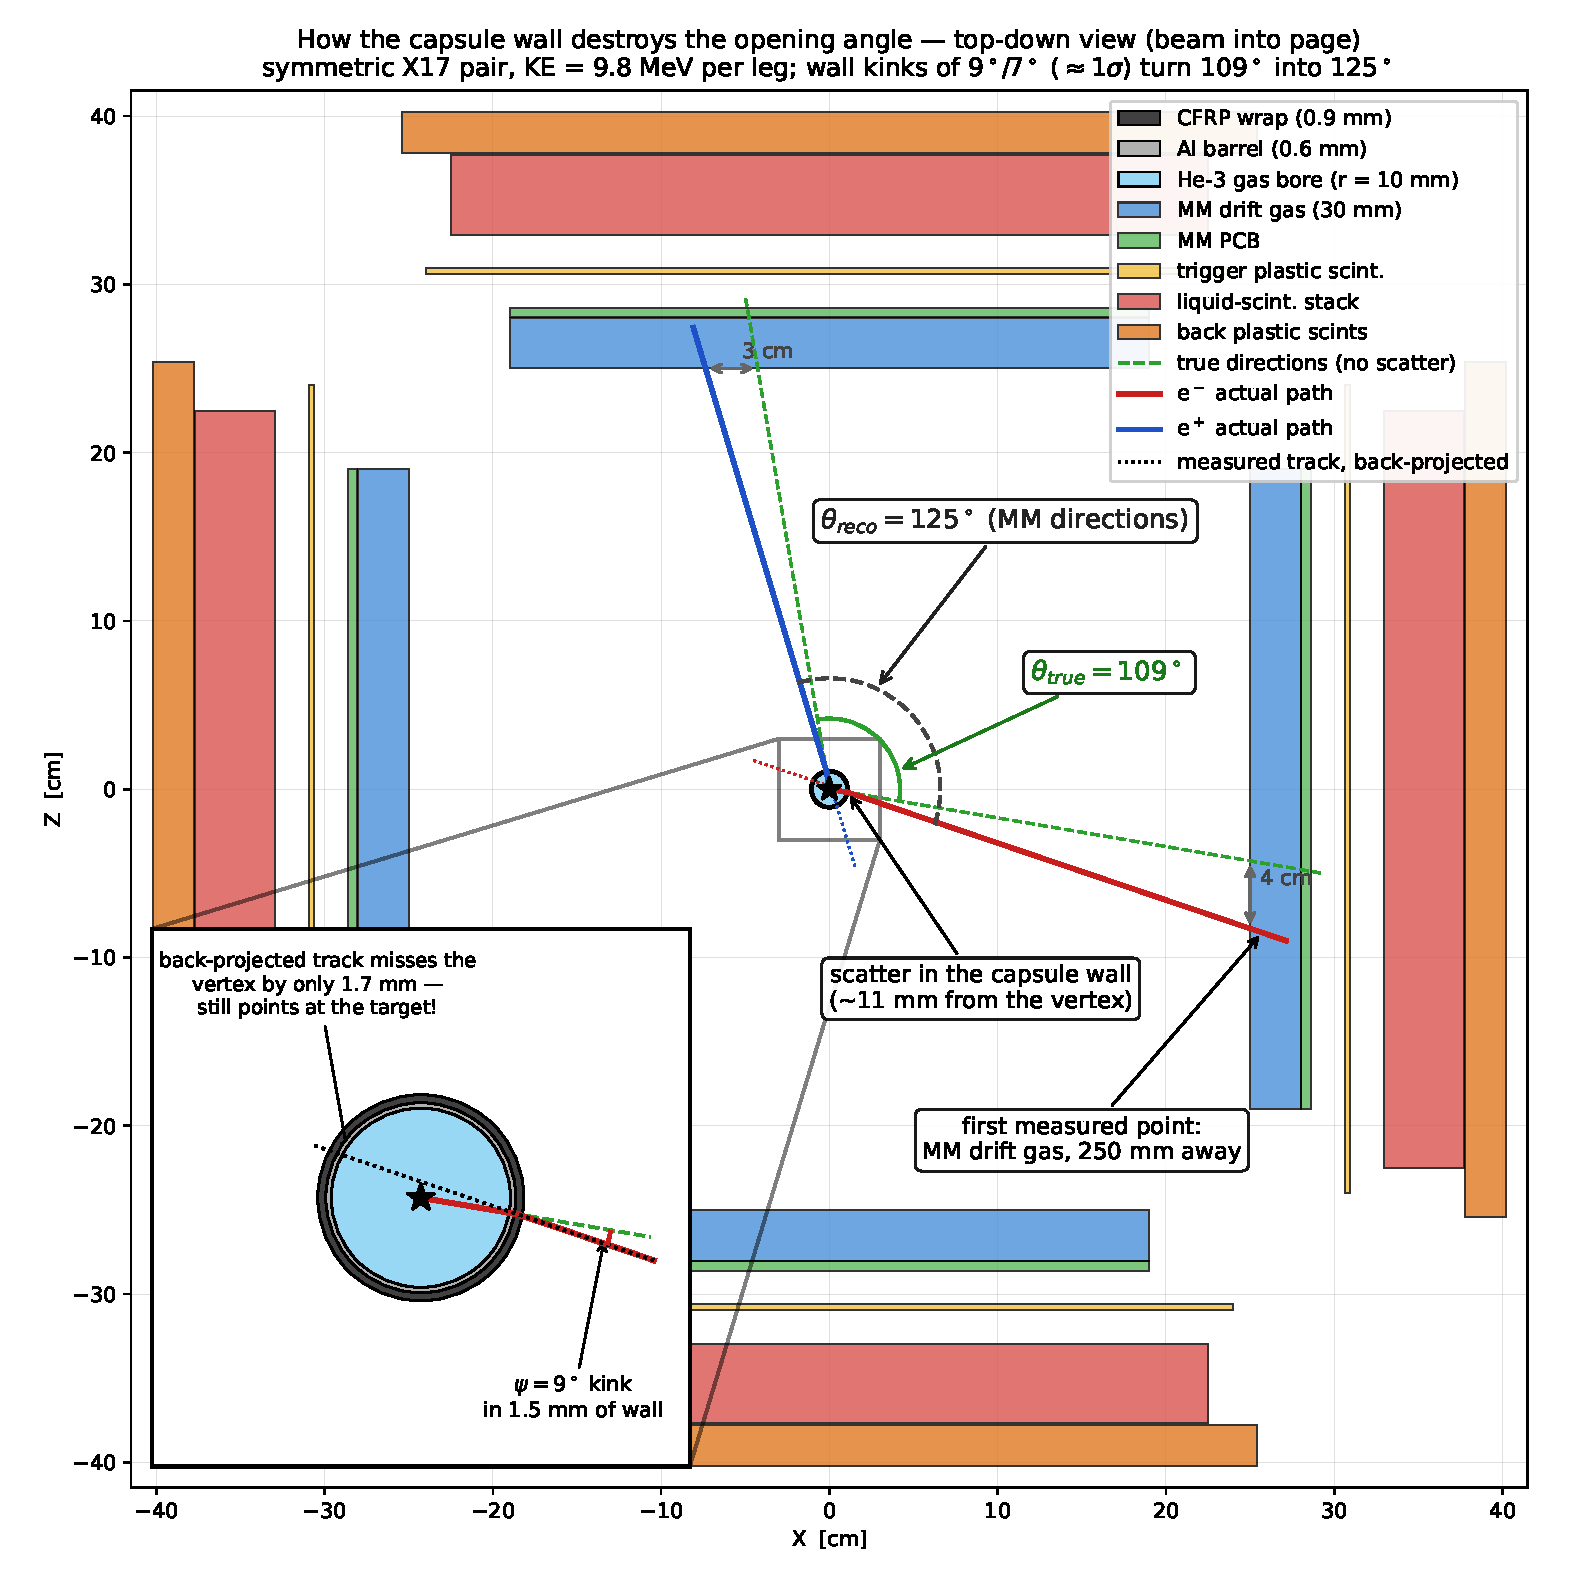
\includegraphics[width=0.92\textwidth]{fig_ang_diagram.pdf}
\end{center}

\noindent The picture above is the whole result. Both legs of the pair
scatter in the capsule wall --- 0.6\,mm of Al plus 0.9\,mm of CFRP, crossed
$\sim$11\,mm from the vertex --- by a typical (Highland)
$\theta_0 \approx 7^{\circ}$ \emph{per leg} at the energies of a symmetric
X17 pair. Everything downstream of that wall measures the \emph{kinked}
directions perfectly well, and reconstructs the wrong opening angle. The
zoom shows why no constraint can repair it: the kink happens so close to the
origin that the back-projected track still passes within $\sim$2\,mm of the
vertex --- \textbf{the scattered event remains fully consistent with ``a pair
from the target''}. Quantitatively, for the full accepted spectrum
($\sig{}$ = half the 16--84\% span of
$\dth = \theta_{\mathrm{reco}}-\theta_{\mathrm{truth}}$):

\begin{center}
\begin{tabular}{lcc}
\toprule
pair-level method & $\sig{}$ X17 & $\sig{}$ IPC \\
\midrule
direction at first MM hit (perfect tracker) & $15.5^{\circ}$ & $15.0^{\circ}$ \\
PCA fit of the drift track ($+0.5$\,mm hit smear) & $16.0^{\circ}$ ($16.5^{\circ}$) & $15.5^{\circ}$ ($15.5^{\circ}$) \\
chord: \textbf{true vertex} $\to$ first MM hit \emph{(oracle)} & $\mathbf{14.5^{\circ}}$ & $\mathbf{13.0^{\circ}}$ \\
chord: target centre $\to$ first MM hit \emph{(realistic)} & $15.0^{\circ}$ & $13.5^{\circ}$ \\
\bottomrule
\end{tabular}
\end{center}

\noindent All seven methods (the remaining three sit between these) land
within $2^{\circ}$ of each other, and the \emph{realistic} vertex-constrained
chord is within $0.5^{\circ}$ of the truth-vertex oracle: with the small
capsule, \textbf{the ``pairs come from the target'' trick is already
implemented and already saturated}. Selecting the most symmetric pairs
(min-leg KE $>8$\,MeV) reaches the plateau $\sig{}\!\approx\!12.5^{\circ}$
($11.5^{\circ}$ oracle) --- the floor. The consequence for the measurement:

\begin{center}
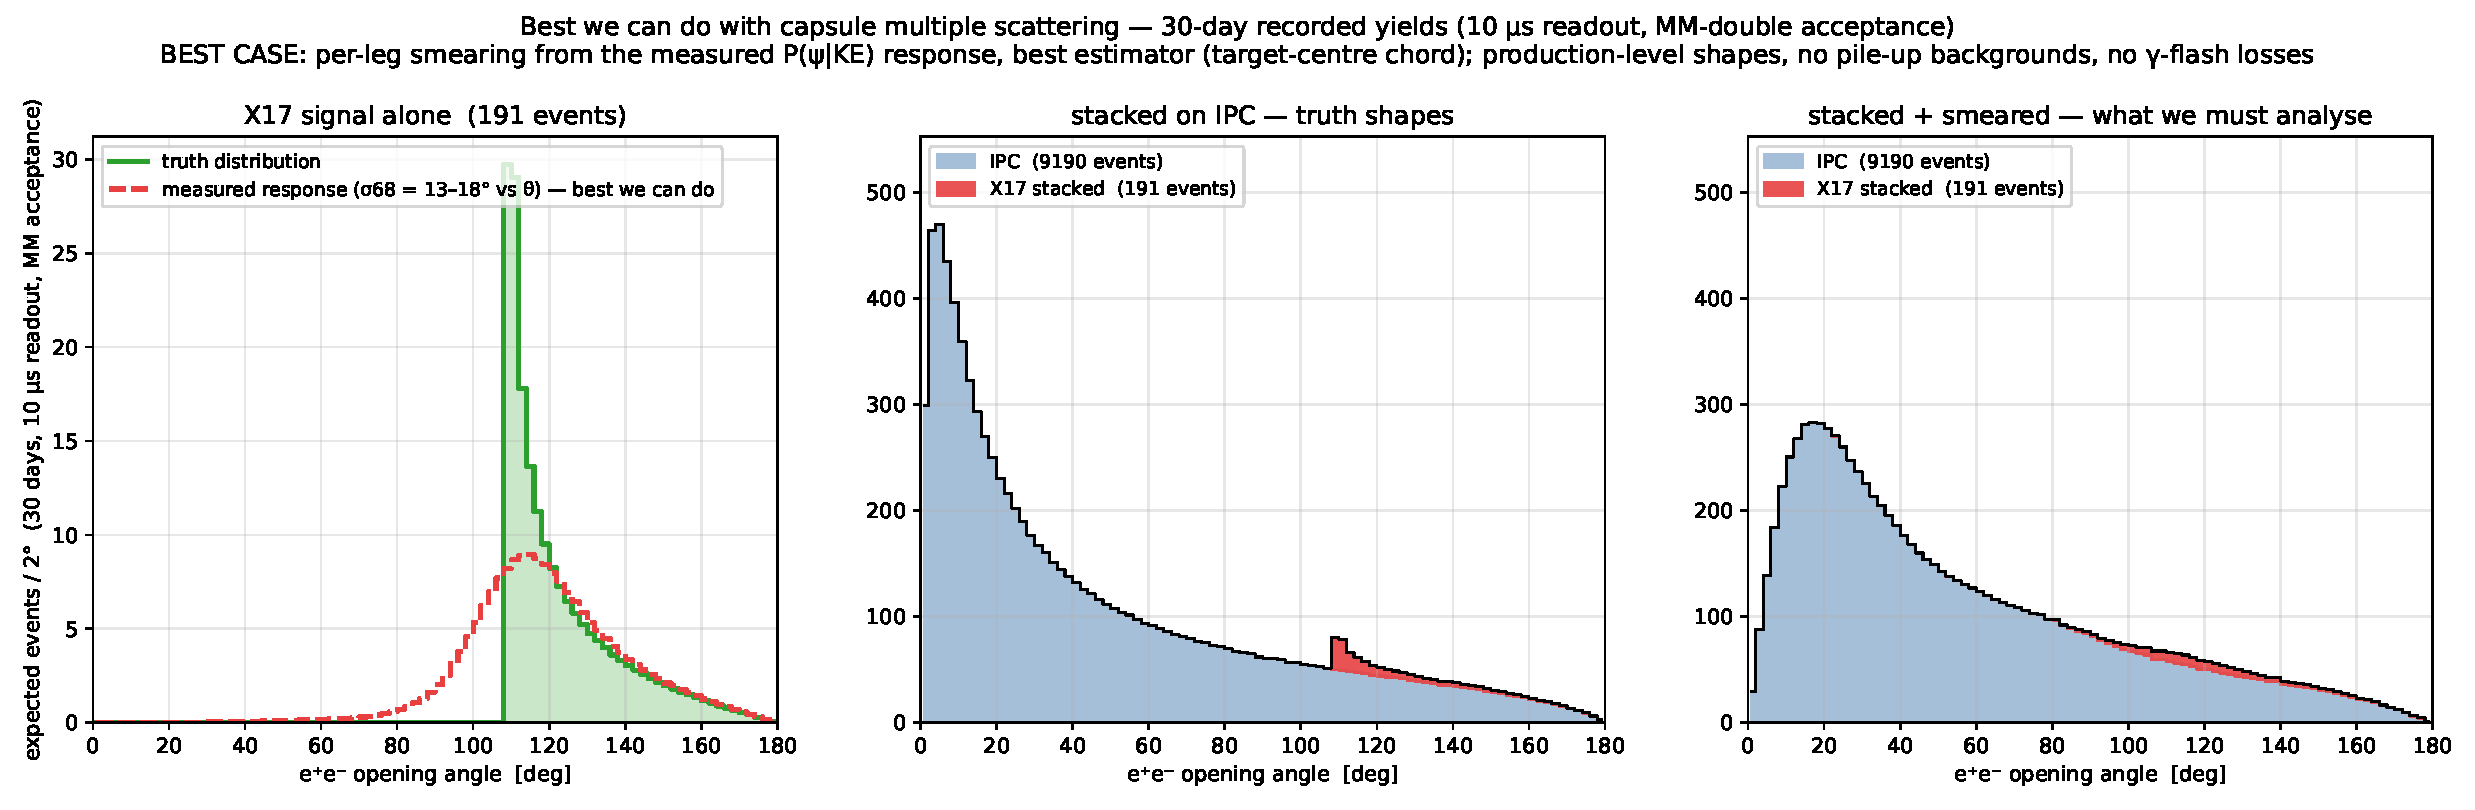
\includegraphics[width=0.99\textwidth]{fig_theta_money.pdf}
\end{center}

\noindent This is the bottom line of the whole study, in expected 30-day
recorded events. \textbf{Left:} the truth X17 distribution --- the sharp
$109^{\circ}$ kinematic shoulder --- against the \emph{best we can do}
given the capsule multiple scattering: each leg's direction smeared with
the full measured $P(\psi\,|\,\mathrm{KE})$ response of the best estimator
(the target-centre chord), so the pair resolution varies with the angle
itself --- $13^{\circ}$ at the shoulder, where pairs are symmetric, growing
to $\sim$18$^{\circ}$ toward $180^{\circ}$ (Fig.~\ref{fig:resvstheta}).
The result is a $\sim$40$^{\circ}$-FWHM bump at a quarter of the height.
\textbf{Middle:} that truth signal stacked on the recorded IPC continuum
--- even unsmeared it is only a $\sim$60\% local excess. \textbf{Right:}
both species smeared --- \emph{this is the spectrum the analysis actually
has to extract the X17 signal from}: a $\lesssim$17\% broad enhancement of
a featureless falling continuum. And
this is a \emph{best-case} picture: smallest feasible smearing, no MM
acceptance shaping, no pile-up backgrounds, no $\gamma$-flash losses.
\textbf{A cut-and-count peak search on the opening angle is dead, with or
without reconstruction improvements.} The resolution is frozen by the wall:
it contributes 79\% of the $x/X_0 = 1.26\%$ upstream budget, the simulation
reproduces the analytic Highland prediction, and the scattering-localization
study places the damage at the wall radius. The MM spatial resolution is
irrelevant (a 0.5\,mm hit smear costs $0.5^{\circ}$).

\subsection*{What can still be done}
In order of leverage (Part II \S7--9):
\begin{enumerate}
\item \textbf{Fit the spectrum, don't cut it.} The response matrix
  $P(\theta_{\mathrm{reco}}\,|\,\theta_{\mathrm{truth}})$ is measured with
  $10^{7}$ events; a template likelihood fit (smeared signal + IPC continuum
  + pile-up backgrounds from the Stage-4 sampler) converts resolution into a
  statistics penalty instead of a veto. The go/no-go number becomes the
  expected significance of that fit with $\sim$190 signal events per 30 days
  --- the natural next study, and the machinery exists.
\item \textbf{MM-internal quality cuts as an energy proxy.} The
  $30$--$40^{\circ}$ tails come from legs below $\sim$3\,MeV. Without
  calorimetry they can still be tagged inside the MM (track straightness,
  drift-gas $dE/dx$, range), buying the $15.5\to12.5^{\circ}$ plateau.
\item \textbf{Bias correction} ($+3.5^{\circ}$ at high KE, larger for soft
  pairs) --- free, automatic in a response-matrix fit.
\item \textbf{Hardware} is the only way below $12^{\circ}$: removing the Al
  barrel (53\% of the budget) scales $\sigma \propto \sqrt{x/X_0}$ to
  $\approx\!0.7\times$, i.e.\ $\sig{}\approx10^{\circ}$.
  Fig.~\ref{fig:dilution} (\S8) shows this does \emph{not} qualitatively
  change the picture.
\end{enumerate}

\noindent\textbf{The bottom line: the opening-angle resolution is
hardware-limited at $\sig{} \approx 12$--$15^{\circ}$ by $\sim$1.5\,mm of
capsule wall sitting 11\,mm from the vertex, every reconstruction trick
including the target-vertex constraint is already within $\sim$1$^{\circ}$ of
its theoretical bound, and the X17 angular peak does not survive as a visible
bump. If the experiment is recoverable, it is recoverable at the
spectrum-fit level, not the event level} --- quantifying that fit is the
follow-on study this note motivates.

%=============================================================================
\clearpage
\section*{Part II --- The full story}

\section{The measurement this note is about}

The DAQ records a fixed $\sim$10\,$\mu$s readout per pulse starting at the
EAR2 $\gamma$ flash (no scintillator trigger; the 0.2--2\,MeV core of the
production arrives 1.0--3.2\,$\mu$s in, and the readout reaches
$E_n \approx 20$\,keV). The working assumption for this note --- pending the
flash-recovery measurement --- is that the liquid-scintillator calorimetry is
saturated and contributes nothing event-by-event. What remains per pair is
geometry: two charged tracks in the MM arms. From two directions one can form
exactly one discriminating quantity, the opening angle $\theta$. For a decay
$X17\to e^+e^-$ the invariant mass obeys
\begin{equation}
m^2 = 2m_e^2 + 2\left(E_+E_- - p_+p_-\cos\theta\right),
\end{equation}
so with energies unmeasured, $\theta$ carries all the mass information we
will ever get. For an at-rest capture ($E^{*}=20.58$\,MeV) the X17 signal
populates $\theta \ge \theta_{\min} = 2\arcsin(16.8/20.58) = 109.4^{\circ}$,
with a sharp shoulder at the threshold (symmetric pairs) and a tail to
$180^{\circ}$ (asymmetric pairs). IPC fills a smooth continuum. The
experiment's discriminating power is therefore set by one number: how well
$\theta$ is reconstructed. For scale: near the shoulder,
$dm/d\theta \approx (E^{*}/2)\cos(\theta/2) \approx 0.10$\,MeV/deg, so a
$15^{\circ}$ angular error is the mass-equivalent of $\pm1.6$\,MeV --- but
only for symmetric pairs; for the rest, the unknown energy sharing already
smears the $\theta\leftrightarrow m$ map before the detector does anything.

\section{Anatomy of a measured pair}

The summary diagram (Part I) shows one worked event in the true top-down
geometry: a symmetric X17 pair (9.8\,MeV kinetic energy per leg), vertex at
the capsule centre, one leg toward the $+X$ arm and one toward the $+Z$ arm.
Each leg crosses $\sim$10\,mm of 500-bar \He{3}, then 0.6\,mm of aluminium
and 0.9\,mm of CFRP, then 24\,cm of air, and is first \emph{measured} in the
MM drift gas at 250\,mm. The wall crossing deflects each leg by a random
angle of Highland width $\theta_0 \approx 7^{\circ}$ (at this energy; much
worse for softer legs). In the diagram the kinks are drawn at their actual
$\approx\!1\sigma$ values, $9^{\circ}$ and $7^{\circ}$: the measured opening
angle becomes $125^{\circ}$ instead of $109^{\circ}$, and the hits arrive
3--4\,cm away from where the unscattered tracks would have landed.

Figure~\ref{fig:gallery} repeats the identical true pair under three throws
of the scattering dice. The same $109^{\circ}$ event is reconstructed at
$97^{\circ}$, $121^{\circ}$, or $134^{\circ}$ --- a spread comparable to the
full width of the physical signal region. Figure~\ref{fig:fan} shows the
same fact as an ensemble: the 68\%/95\% cones each track can occupy after
the wall, and the distribution that one single true angle becomes. Already
this idealized toy --- two legs, Gaussian $\theta_0=7.1^{\circ}$ each,
nothing else --- gives $\sig{} = 9.8^{\circ}$. The full Geant4 answer for
such symmetric pairs is $11.5$--$12.5^{\circ}$ (non-Gaussian MS tails,
oblique wall crossings, drift-gas scattering), growing to
$14.5$--$15.5^{\circ}$ over the whole accepted spectrum because one leg of
an X17 pair is always below $9.8$\,MeV and $\theta_0 \propto 1/p$.

\begin{figure}[htb]
\centering
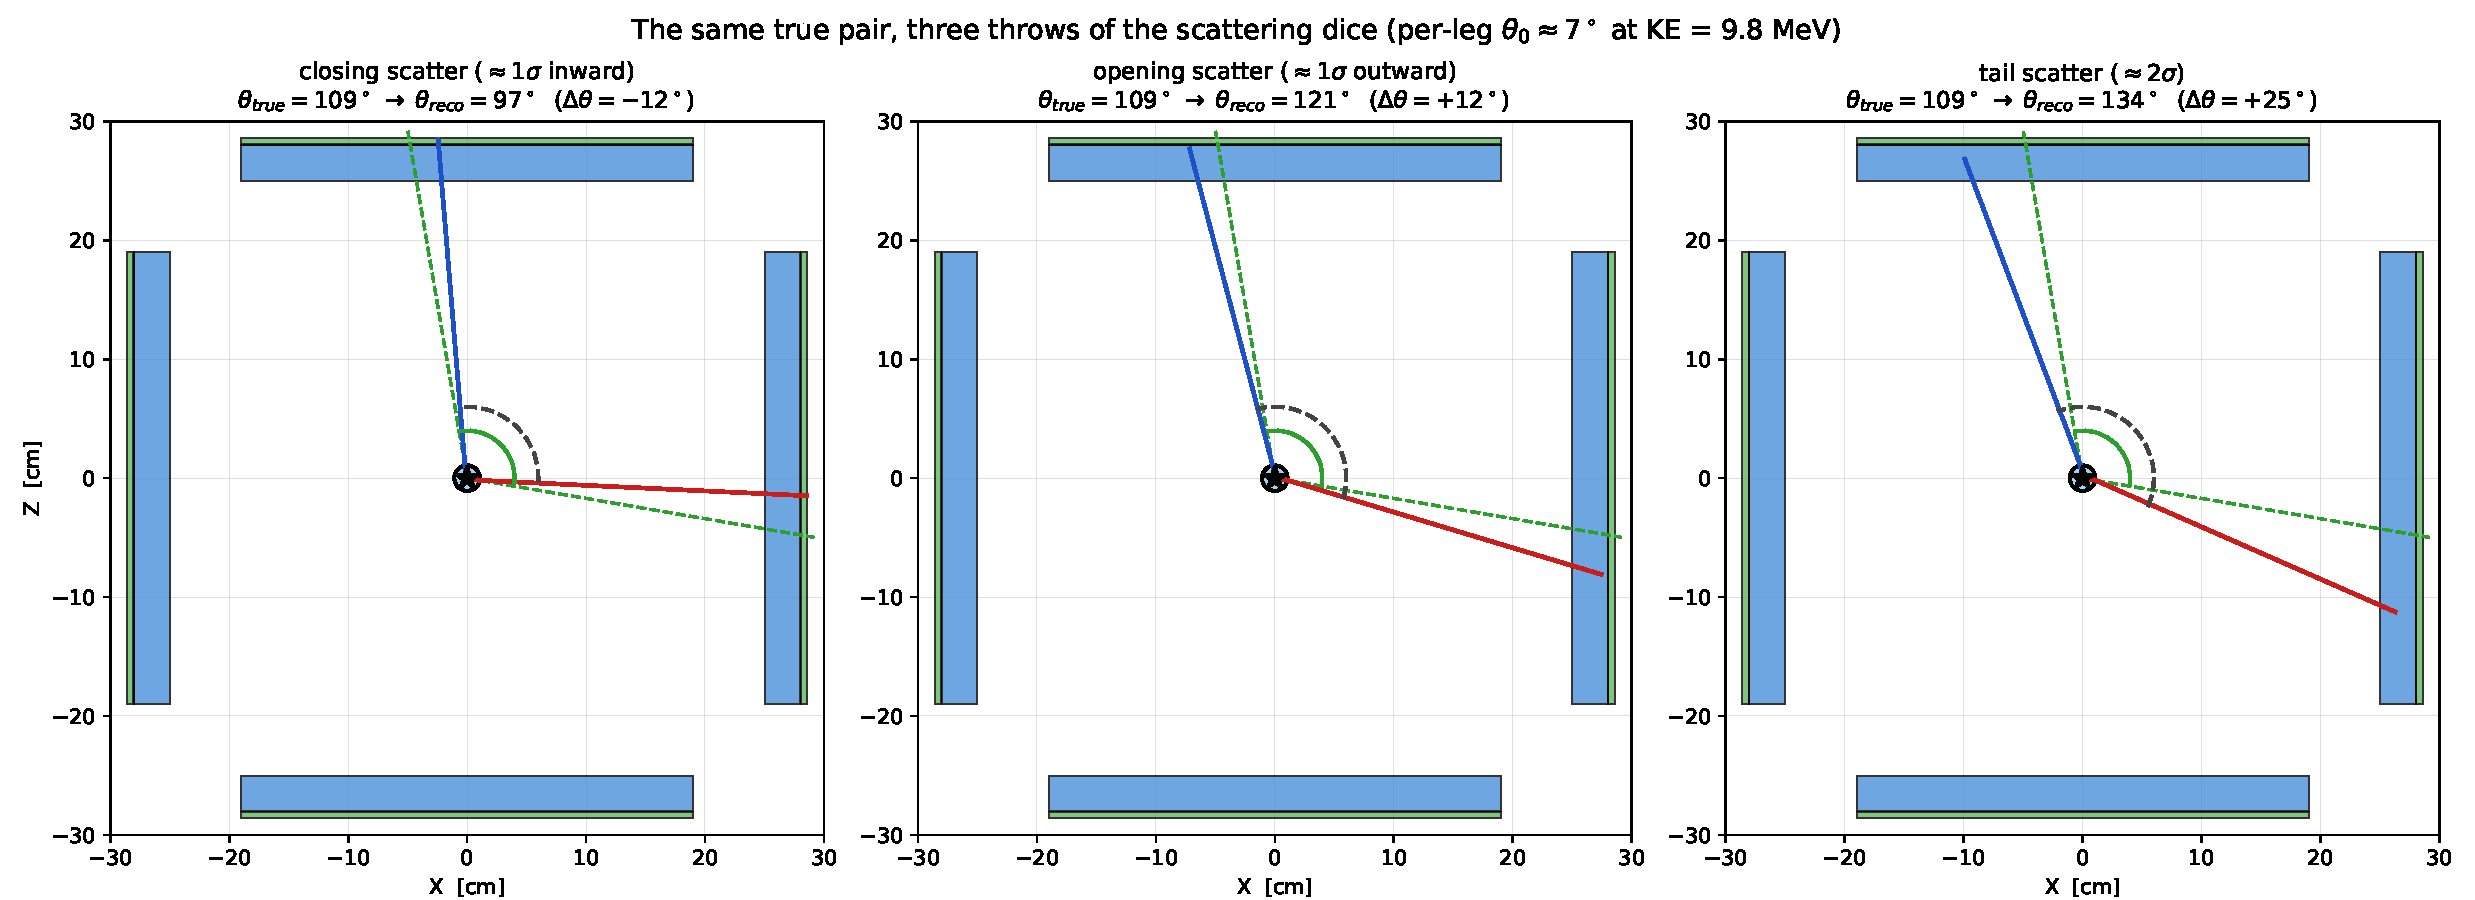
\includegraphics[width=0.99\textwidth]{fig_ang_gallery.pdf}
\caption{One true pair ($\theta_{\mathrm{true}}=109^{\circ}$, symmetric),
three scattering outcomes drawn in the real geometry (MM drift gas in blue;
downstream stack omitted for clarity). Green dashed: unscattered paths.
The wall kink is invisible at the capsule scale --- see the Part-I zoom ---
but dominates the reconstructed angle 250\,mm later.}
\label{fig:gallery}
\end{figure}

\begin{figure}[htb]
\centering
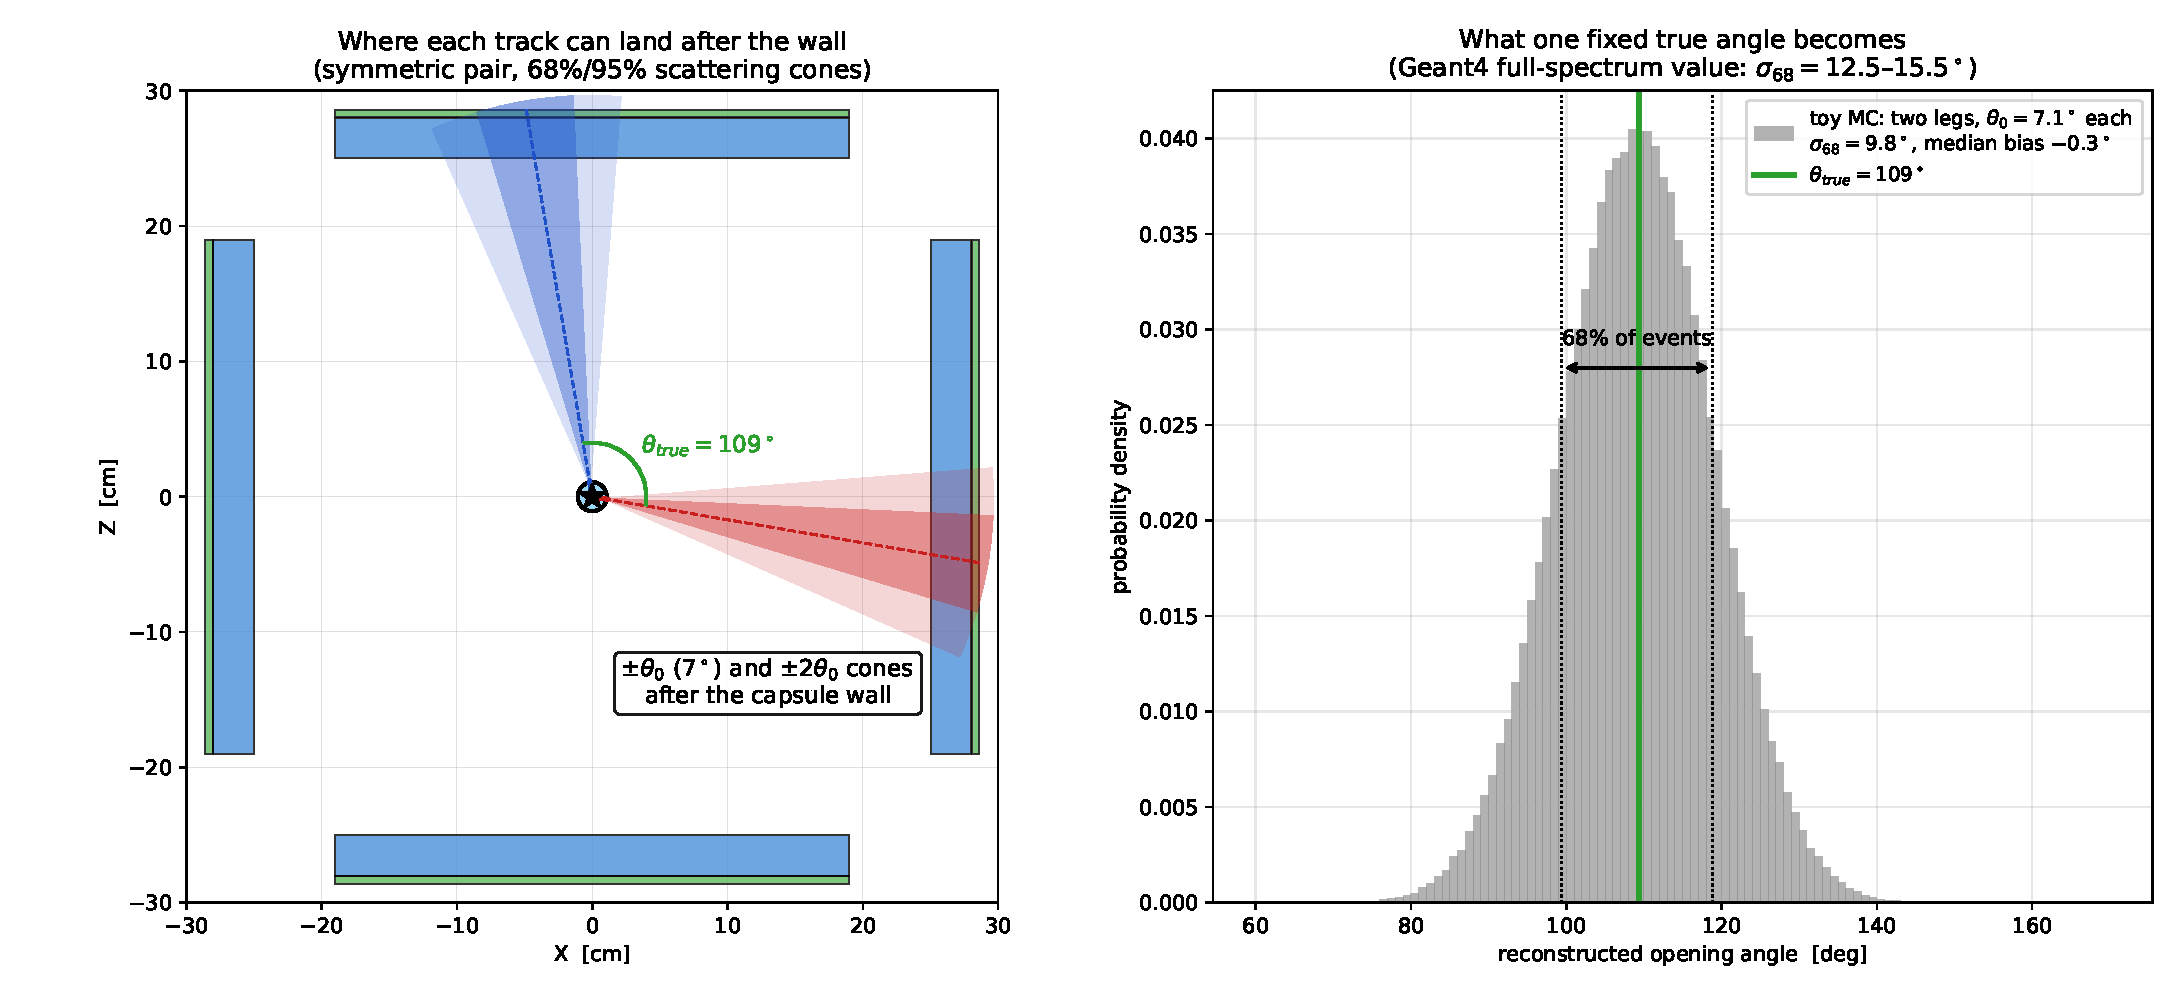
\includegraphics[width=0.99\textwidth]{fig_ang_fan.pdf}
\caption{Left: the 68\%/95\% cones available to each leg of a symmetric pair
after the capsule wall. Right: the opening-angle distribution that a single
fixed $109.4^{\circ}$ pair becomes in a toy MC with only the wall scattering
($\theta_0 = 7.1^{\circ}$ per leg, Gaussian) --- $\sig{}=9.8^{\circ}$ before
any detector effect. The full simulation gives $12.5$--$15.5^{\circ}$.}
\label{fig:fan}
\end{figure}

\section{The estimator catalogue}

Nine per-particle direction estimators and seven pair-level methods were
implemented in \texttt{scripts/analyze\_pairs.py} and evaluated on the
$10^{7}$-event sample. Per particle, $\psi$ is the space angle between the
estimated direction and the truth direction at the vertex:

\begin{center}
\footnotesize
\begin{tabular}{llcc}
\toprule
estimator & what it tests & med.\ $\psi$ (all KE) & KE $>8$\,MeV \\
\midrule
dir.\ at 1st MM hit & upstream MS only --- perfect tracker & $10.4^{\circ}$ & $7.9^{\circ}$ \\
dir.\ at last MM hit / 1st-vs-last & adds / isolates drift-gas MS & \multicolumn{2}{c}{(small; PDF \S13)} \\
PCA fit of drift hits & realistic track fit & $10.4^{\circ}$ & $7.9^{\circ}$ \\
PCA fit vs 1st-hit dir. & fit-method error alone & \multicolumn{2}{c}{($\ll$ MS; PDF \S13)} \\
chord: true vtx $\to$ 1st hit & oracle vertex constraint & $9.4^{\circ}$ & $7.1^{\circ}$ \\
chord: true vtx $\to$ edep centroid & centroid vs first-hit choice & $9.4^{\circ}$ & $7.1^{\circ}$ \\
chord: \textbf{target centre} $\to$ 1st hit & \textbf{realistic vertex constraint} & $9.9^{\circ}$ & $7.9^{\circ}$ \\
chord: vtx $\to$ trig-scint hit ($\sigma$=3\,cm) & scintillator fallback & $11.4^{\circ}$ & $9.4^{\circ}$ \\
\bottomrule
\end{tabular}
\end{center}

\noindent and at pair level ($\sig{}$ of $\dth$, full accepted sample;
overall RMS for the first method is $19.1^{\circ}$/$20.6^{\circ}$ X17/IPC):

\begin{center}
\small
\begin{tabular}{lcc}
\toprule
pair method & X17 & IPC \\
\midrule
dir.\ at 1st MM hit (current default) & $15.5^{\circ}$ & $15.0^{\circ}$ \\
PCA drift-track fit & $16.0^{\circ}$ & $15.5^{\circ}$ \\
PCA fit + 0.5\,mm hit smear & $16.5^{\circ}$ & $15.5^{\circ}$ \\
chord: true vertex $\to$ 1st hit (oracle) & $14.5^{\circ}$ & $13.0^{\circ}$ \\
chord: true vertex $\to$ drift centroid & $14.5^{\circ}$ & $13.5^{\circ}$ \\
chord: target centre $\to$ 1st hit & $15.0^{\circ}$ & $13.5^{\circ}$ \\
chord: vertex $\to$ trigger-scint hit & $15.5^{\circ}$ & $15.0^{\circ}$ \\
\bottomrule
\end{tabular}
\end{center}

Three structural facts stand out. \emph{(i)} The PCA fit gains nothing over
the single first-hit direction: averaging the drift hits removes fit noise
but integrates drift-gas scattering, and the two cancel. \emph{(ii)} A
0.5\,mm hit smear --- a pessimistic MM cluster resolution --- costs only
$0.5^{\circ}$: \textbf{detector granularity is irrelevant}; even mm-scale
resolution would not move the result. \emph{(iii)} Every estimator converges
to the same upstream-MS floor (Fig.~\ref{fig:psi}); the floor itself tracks
the analytic Highland curve of the material budget.

\begin{figure}[htb]
\centering
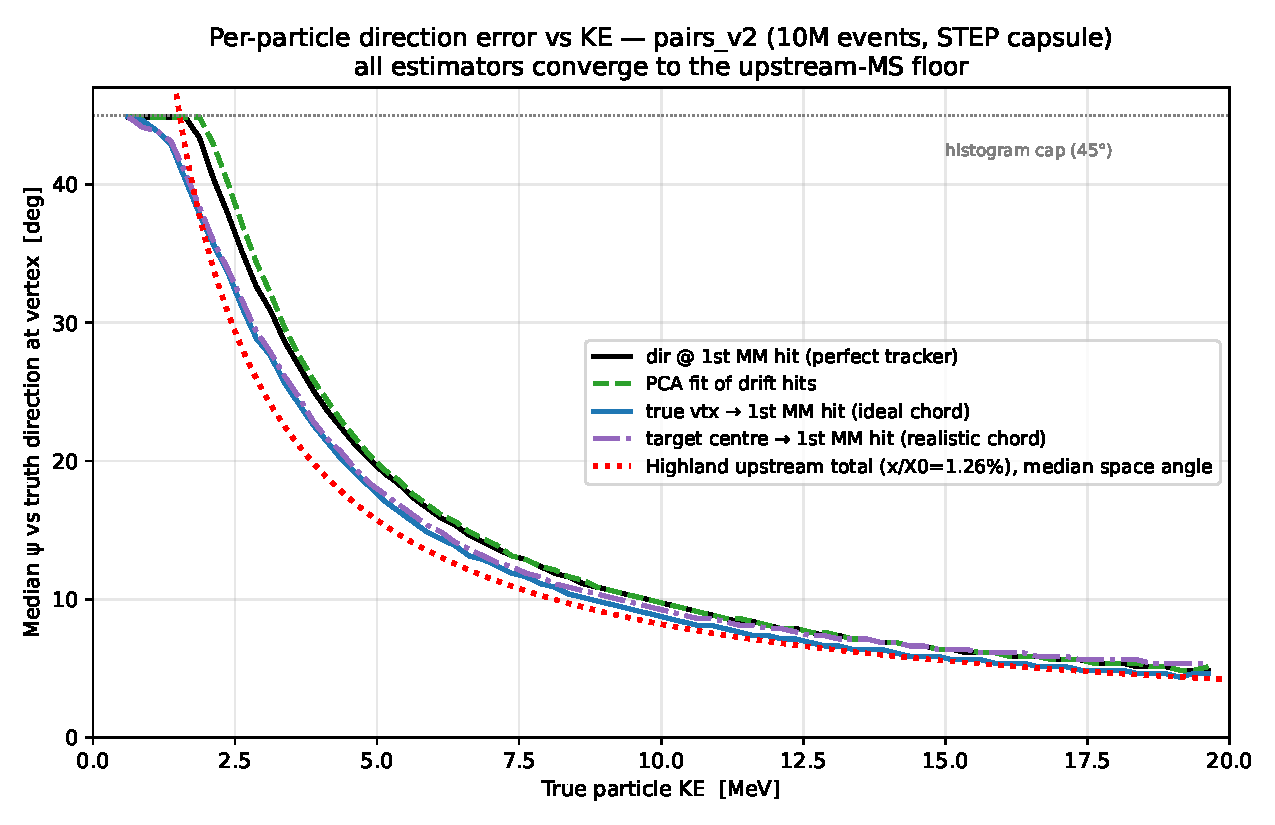
\includegraphics[width=0.78\textwidth]{fig_psi_vs_ke.pdf}
\caption{Median per-particle direction error vs kinetic energy for the four
exported estimators, against the Highland prediction for the full upstream
budget. Below $\sim$2\,MeV the histogram saturates at its $45^{\circ}$ cap
--- such legs are effectively directionless.}
\label{fig:psi}
\end{figure}

\section{Where the angle is lost: the material budget}

The plane-projected Highland width for a singly charged particle crossing
$x/X_0$ radiation lengths is
\begin{equation}
\theta_0 \;=\; \frac{13.6\,\mathrm{MeV}}{\beta c p}\,
\sqrt{x/X_0}\,\bigl[1 + 0.038 \ln (x/X_0)\bigr],
\label{eq:highland}
\end{equation}
and the median \emph{space} angle for Gaussian MS is
$\sqrt{2\ln 2}\,\theta_0 \approx 1.18\,\theta_0$. Evaluating
Eq.~\ref{eq:highland} layer by layer along the radial exit path
(Fig.~\ref{fig:budget}):

\begin{center}
\small
\begin{tabular}{lrrr}
\toprule
layer & $x/X_0$ & share & $\theta_0$ at $p=10$\,MeV$/c$ \\
\midrule
\He{3} gas, 500\,bar, $\sim$10\,mm path & 0.089\% & 7\% & $1.7^{\circ}$ \\
\textbf{Al barrel, 0.6\,mm}             & \textbf{0.674\%} & \textbf{53\%} & $\mathbf{5.2^{\circ}}$ \\
\textbf{CFRP wrap, 0.9\,mm}             & \textbf{0.327\%} & \textbf{26\%} & $\mathbf{3.5^{\circ}}$ \\
air gap, $\sim$23.9\,cm                 & 0.078\% & 6\% & $1.6^{\circ}$ \\
MM window + cathode (Mylar/Kapton/Cu)   & 0.094\% & 7\% & $\le 1.4^{\circ}$ \\
\midrule
\textbf{total upstream}                 & \textbf{1.26\%} & & $\mathbf{7.3^{\circ}}$ \\
\bottomrule
\end{tabular}
\end{center}

\noindent The measured first-hit direction error at KE $\approx 10$\,MeV
($7.9^{\circ}$, Fig.~\ref{fig:psi}) sits on this prediction, and the
scattering-localization study in the analysis PDF (effective single-scatter
distance $s_{\mathrm{eff}} = t - \delta/\tan\psi$) independently places the
median scatter at the wall radius. So the chain of evidence closes: the
resolution is the wall, the wall is $\sim$80\% of the budget, and simulation
and analytic model agree. Note what is \emph{not} on the list: the 500-bar
gas itself (7\%), the air (6\%), and every MM material ($\le$7\% combined).
Pressure is innocent; the \emph{pressure vessel} is guilty.

\begin{figure}[htb]
\centering
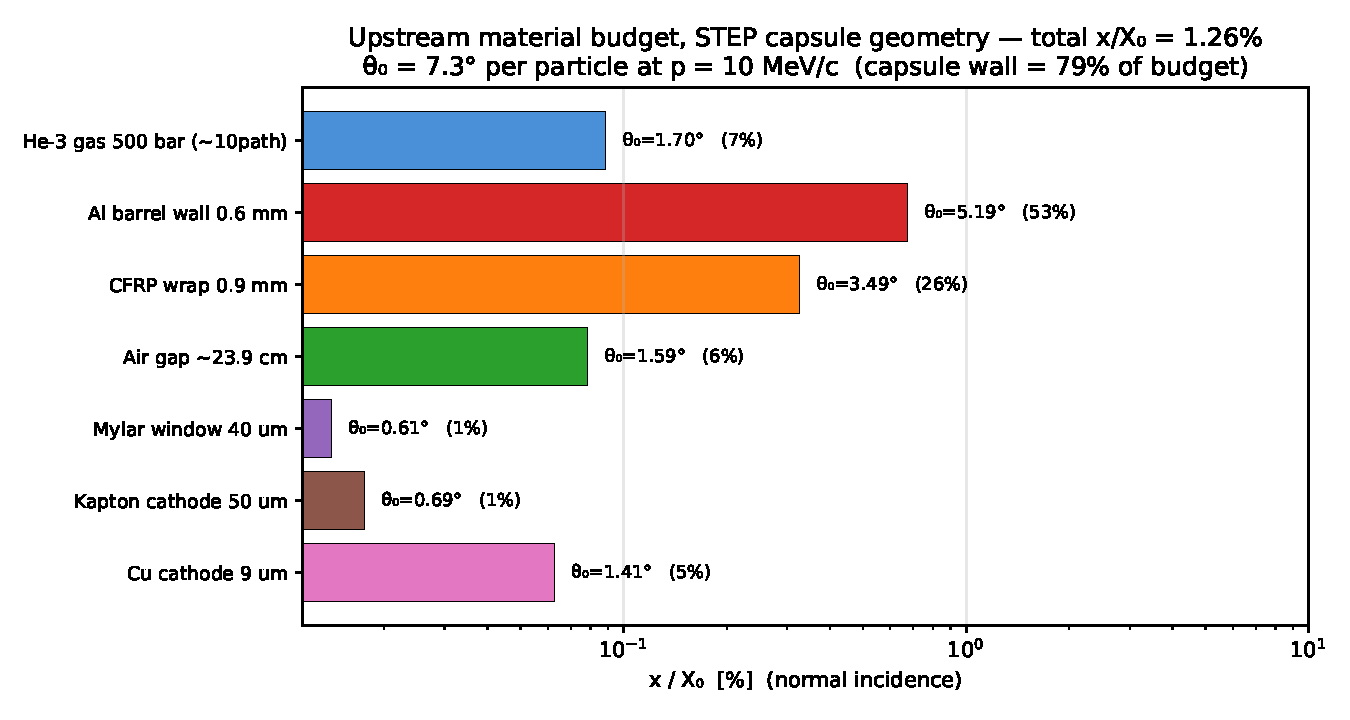
\includegraphics[width=0.8\textwidth]{fig_ms_budget.pdf}
\caption{Upstream material budget for the STEP capsule geometry.}
\label{fig:budget}
\end{figure}

\section{Why the vertex constraint is already exhausted}

The target-as-vertex idea is geometrically sound and is implemented (the
``target centre $\to$ first hit'' chord). The reason it buys so little is
worth stating precisely, because it also rules out every variant of the
idea.

\textbf{(a) The chord inherits the scatter.} A kink $\psi$ at distance $s$
from the vertex displaces the track at the measurement plane $L$ by
$(L-s)\tan\psi$; the chord from the vertex to that point therefore makes an
angle $\psi\,(L-s)/L$ with the true initial direction. With $s\approx11$\,mm
and $L=250$\,mm, the chord retains $0.956\,\psi$. That 4\% rebate is the
entire $\sim$1$^{\circ}$ oracle improvement seen in the tables.

\textbf{(b) Moving the tracker closer makes it worse.} The chord error
$\to 0$ as $L \to s$, so a measurement plane just outside the wall plus a
vertex would recover the true direction --- but the vertex is unknown within
the capsule (RMS $\approx$16\,mm along the beam, $\approx$5\,mm
transverse), adding $\sigma_v/L$ to the chord. At $L=250$\,mm that costs
$\sim$3$^{\circ}$ (measured: the realistic chord is $3.1^{\circ}$ in
quadrature above the oracle); at $L=50$\,mm it would cost $>10^{\circ}$.
Short lever arms lose more to vertex ignorance than they gain on the
scatter; the current 250\,mm is already near the optimum.

\textbf{(c) The event cannot tell you its own vertex.} Back-projected
tracks miss the true vertex by a median of 1.0\,cm (KE 10--15\,MeV) to
3.7\,cm (3--4\,MeV) --- at or beyond the 10\,mm bore radius. A two-track
vertex fit is therefore \emph{weaker} than the prior ``somewhere in the
capsule''; equivalently, the Part-I zoom shows the scattered track still
pointing at the target. Pointing cuts keep their value for background
rejection, but carry no information to correct the angle with.

Together (a)--(c) bound every vertex-flavoured scheme: chords, constrained
fits, vertex refits, extra tracking layers. With the small capsule the
realistic chord sits $0.5^{\circ}$ from the truth-vertex oracle, and the
oracle sits $1^{\circ}$ from the perfect tracker. \textbf{Total theoretical
headroom from smarter geometry-based reconstruction:
$\lesssim 1.5^{\circ}$.}

\section{What cannot work at all without calorimetry}

A kinematic fit is the standard rescue when a constraint is unused, so we
checked the counting explicitly. Unknowns per event: the two momentum
magnitudes (directions are measured). Available at-rest-capture constraints:
energy conservation ($E_+ + E_- = 20.58$\,MeV) and the fixed parent momentum
($|\vec p_+ + \vec p_-| = 11.9$\,MeV$/c$). Imposing \emph{both} solves for
the two magnitudes --- but then
$m^2 = (E_++E_-)^2 - |\vec p_+ + \vec p_-|^2$ is fixed to $16.8$\,MeV
identically, independent of the data: the fit returns its own hypothesis.
Imposing only one leaves one equation for two unknowns. There is no middle
ground: \textbf{without an energy measurement there is no per-event mass and
no kinematic sharpening of $\theta$.} The opening angle, as smeared by the
wall, is the final observable.

\section{What still can be done, with expected gains}

\begin{figure}[htb]
\centering
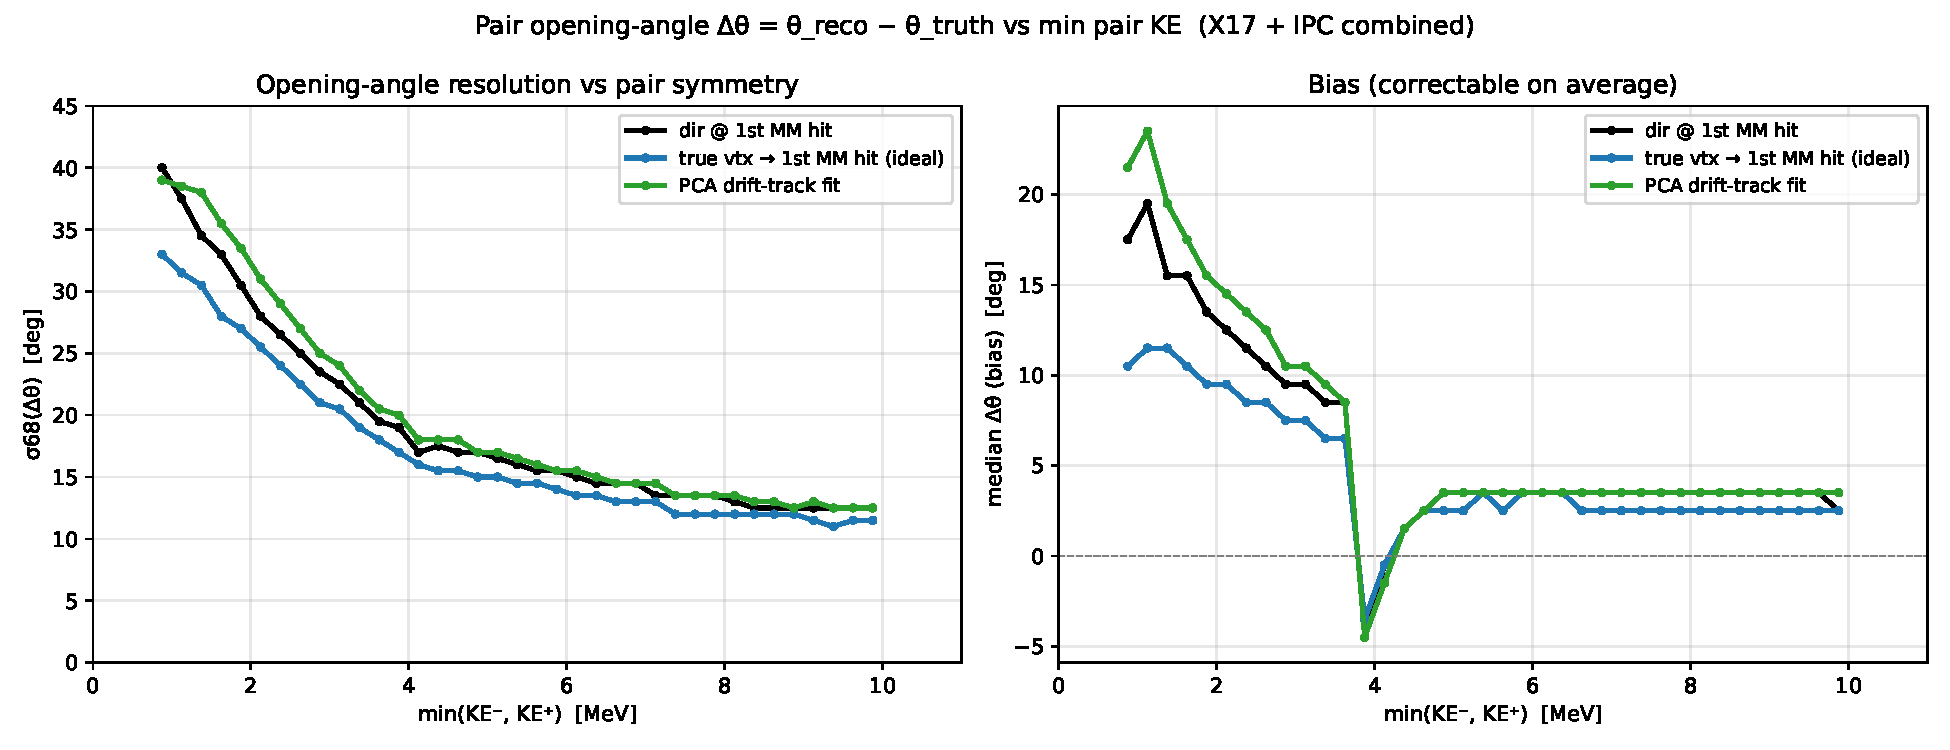
\includegraphics[width=0.95\textwidth]{fig_sigma68_vs_minke.pdf}
\caption{Resolution and bias vs the softer leg's kinetic energy. The plateau
above $\sim$8\,MeV is the symmetric-pair floor; the soft-leg events supply
the long tails. (The bias spike at $\sim$4\,MeV is a quantile/binning
artifact of a bimodal residual, not physics.)}
\label{fig:minke}
\end{figure}

\begin{enumerate}
\item \textbf{Template fit of the $\theta$ spectrum} (the main path). The
  measured response $P(\theta_{\mathrm{reco}}|\theta_{\mathrm{truth}})$,
  including its bias and non-Gaussian tails, is in
  \texttt{analysis/pairs\_v2/geant4\_response.json} and already loads into
  the \texttt{MX17\_Simulation} fast-MC. A binned likelihood fit of
  signal$+$background templates uses the full shape information; resolution
  degrades the \emph{statistical power} smoothly instead of erasing the
  peak. The required follow-on study: expected significance vs run time,
  with the IPC continuum and the Stage-4 pile-up backgrounds under the
  realistic response. Until that number exists, the experiment is neither
  dead nor alive.
\item \textbf{MM-internal soft-leg rejection.} Fig.~\ref{fig:minke}: cutting
  the soft legs moves $15.5^{\circ}\!\to\!12.5^{\circ}$ and removes the worst
  tails (and the worst bias). The study above used \emph{truth} KE; the open
  task is to build the proxy from MM-only quantities (drift $dE/dx$, track
  straightness, range/penetration) and measure its efficiency--purity. Soft
  legs are also the most-scattered legs, so the proxy tags exactly what we
  want to remove.
\item \textbf{Bias correction:} $+2.5$--$3.5^{\circ}$ on the plateau, tens of
  degrees for soft pairs --- absorbed automatically by item 1.
\item \textbf{Statistical micro-gains:} per-event vertex-$y$ estimate from
  the two hit positions, optimal chord$+$direction combination ---
  $\lesssim 0.5^{\circ}$ combined, bounded by \S5.
\end{enumerate}

\section{The hardware ceiling}

If a future capsule iteration is on the table, $\sigma \propto
\sqrt{x/X_0}$ sets the exchange rate:

\begin{center}
\small
\begin{tabular}{lccc}
\toprule
change & upstream $x/X_0$ & $\sigma$ scale & full-spectrum $\sig{}$ \\
\midrule
current (Al 0.6\,mm + CFRP 0.9\,mm) & 1.26\% & 1.00 & $15.5^{\circ}$ \\
halve both walls & 0.76\% & 0.78 & $12^{\circ}$ \\
remove Al barrel (all-composite vessel) & 0.59\% & 0.68 & $10.5^{\circ}$ \\
remove the wall entirely (unphysical) & 0.26\% & 0.45 & $7^{\circ}$ \\
\bottomrule
\end{tabular}
\end{center}

\begin{figure}[htb]
\centering
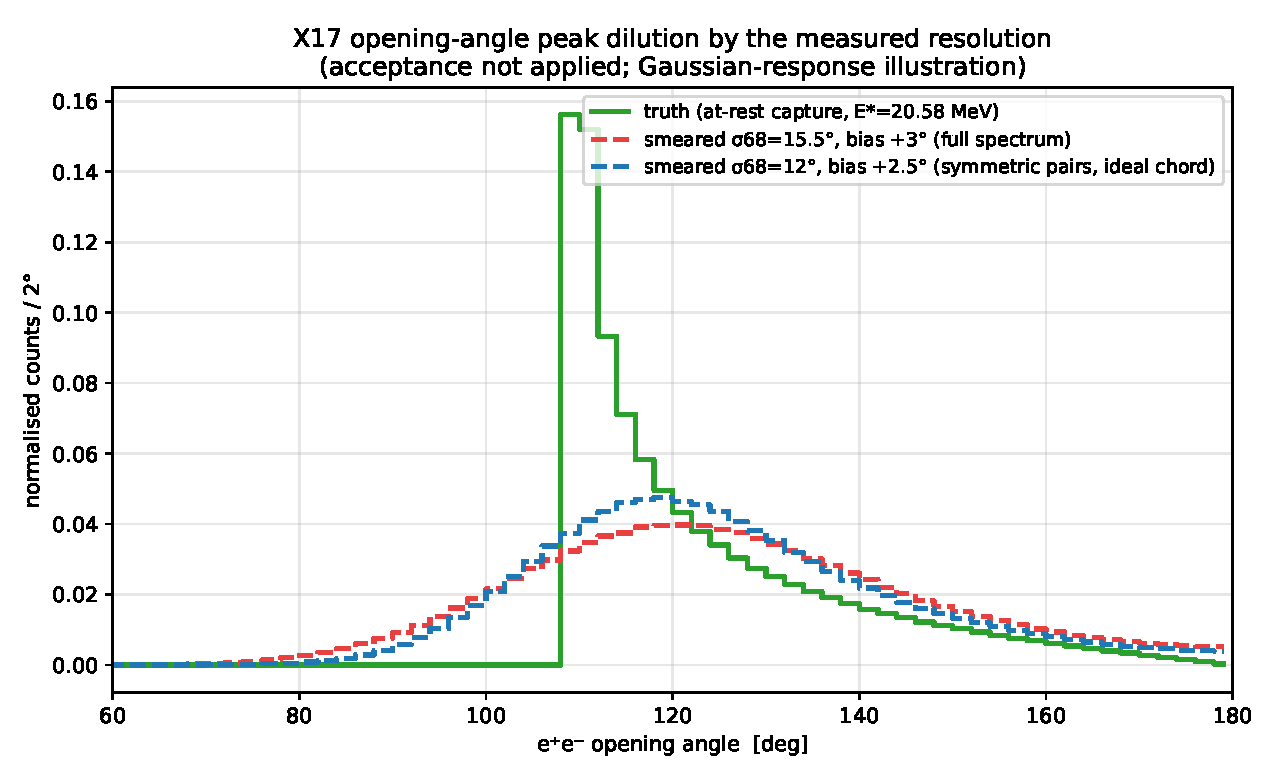
\includegraphics[width=0.78\textwidth]{fig_theta_dilution.pdf}
\caption{The X17 truth spectrum against two smearing scenarios: the current
full-spectrum resolution ($\sig{}=15.5^{\circ}$, red) and the
symmetric-pair/ideal-chord floor ($\sig{}=12^{\circ}$, blue) --- which is
also where the realistic hardware options of the table land. The two
smeared curves are nearly indistinguishable: improving the resolution by
the maximum plausible amount barely changes what is observable.}
\label{fig:dilution}
\end{figure}

\noindent Even the unphysical limit leaves a $7^{\circ}$ smearing of a
shoulder whose physical width is comparable --- and the realistic options
land at $10$--$12^{\circ}$, which Fig.~\ref{fig:dilution} shows is
visually indistinguishable from the present situation. Hardware helps the
template fit; it does not resurrect the visible peak.

\section{Consequences for the X17 search}

\begin{figure}[htb]
\centering
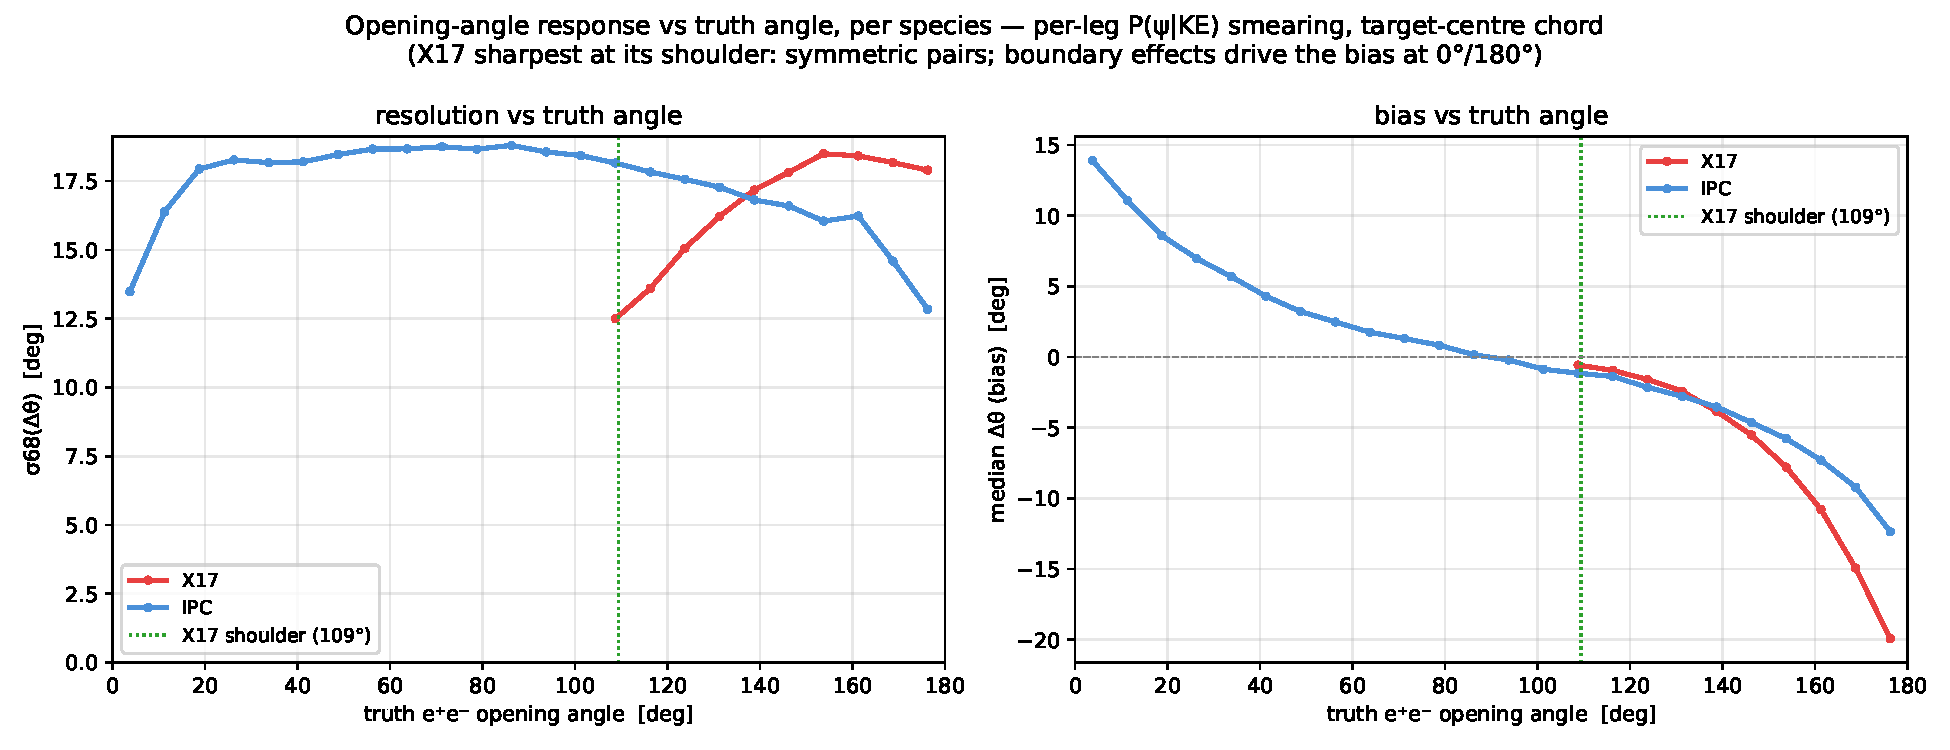
\includegraphics[width=0.95\textwidth]{fig_res_vs_theta.pdf}
\caption{The pair resolution is not flat in $\theta$ --- and it differs
between species. Per-leg response smearing (measured
$P(\psi\,|\,\mathrm{KE})$, target-centre chord) propagated to the pair
level, binned in \emph{truth} opening angle. X17 (red, defined only above
$109^{\circ}$): sharpest at its shoulder ($13^{\circ}$), where pairs are
symmetric and both legs carry $\sim$9.8\,MeV, degrading to
$\sim$18$^{\circ}$ toward $180^{\circ}$ where one leg is soft. IPC (blue):
sharpest at \emph{small} angle ($\sim$13$^{\circ}$ --- low-mass pairs
split $E^{*}$ almost evenly, giving two stiff legs), worst
($\sim$18.5$^{\circ}$) through the $30$--$90^{\circ}$ mid-range. The bias
(right) is driven by the $0^{\circ}$/$180^{\circ}$ boundaries:
$+13^{\circ}$ at small angles, $-10$ to $-20^{\circ}$ near $180^{\circ}$.
The money plot (Part~I) inherits all of this automatically. The mild good
news: the signal region is where the X17 response is \emph{best}.}
\label{fig:resvstheta}
\end{figure}

\begin{figure}[htb]
\centering
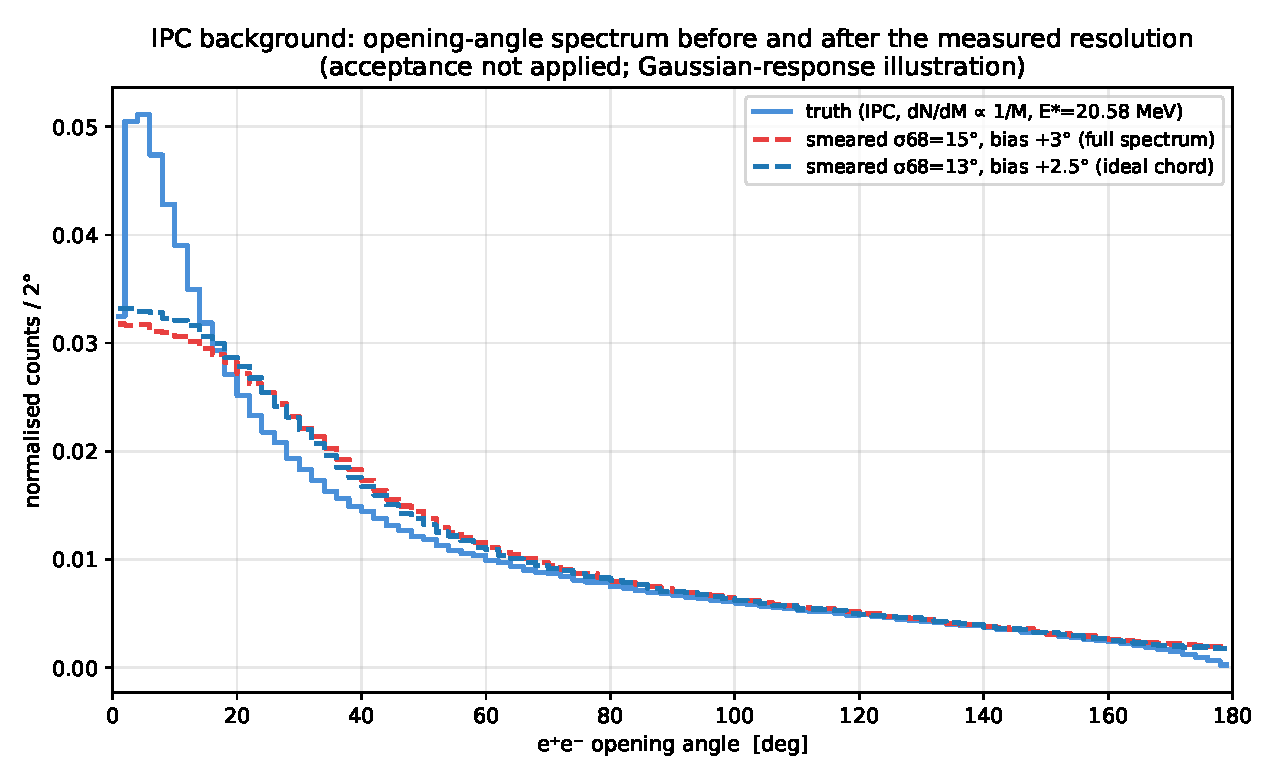
\includegraphics[width=0.74\textwidth]{fig_ipc_dilution.pdf}
\caption{The IPC background spectrum before and after the measured
resolution (same construction as the X17 dilution plot in Part~I; the
virtual-state mass is sampled from the generator's $dN/dM \propto 1/M$).
The one structure IPC has --- the small-angle pile-up from low-mass pairs
--- is flattened, and \emph{everything above $\sim$60$^{\circ}$ is
essentially invariant}: a smooth continuum smeared by $15^{\circ}$ is the
same smooth continuum. The resolution damages only the signal.}
\label{fig:ipcdil}
\end{figure}

Putting the pieces together for a 30-day run under the 10\,$\mu$s readout:
$\sim$190 recorded X17 pairs whose $109^{\circ}$ shoulder is smeared into a
$\sim$40$^{\circ}$-FWHM enhancement, on a recorded IPC continuum $\sim$48
times larger before angle cuts ($S/B \approx 0.021$ --- the trigger-free
readout records the small-angle IPC bulk that the old double-arm trigger
silently removed, so the background grows $\times$9 while the signal grows
$\times$2.3), plus pile-up backgrounds to be quantified by the Stage-4
sampler. The discriminating shape survives only statistically.

Figures~\ref{fig:resvstheta}--\ref{fig:ipcdil} and the money plot in Part~I
put the two species on one axis. Three observations. \emph{(i)} The
response varies with angle and species (Fig.~\ref{fig:resvstheta}), and
favourably so: the X17 response is sharpest exactly at its shoulder, while
the IPC continuum is nearly invariant under the resolution
(Fig.~\ref{fig:ipcdil}) --- the entire information loss is the signal
shoulder. \emph{(ii)} At truth level the stacked signal would stand
$\sim$60\% above the continuum at the shoulder (money plot, middle panel);
after smearing the maximum local excess is $\sim$17\%, spread over
$\sim$40$^{\circ}$ (right panel --- the spectrum the analysis must work
with). \emph{(iii)} Naive counting on these best-case shapes in a
105--150$^{\circ}$ window gives
$S \approx 135$ on $B \approx 1030$ ($S/\sqrt{B} \approx 4.2$ per 30 days,
down from 6.2 unsmeared) --- superficially healthy, but three things eat
into it: an excess of $S/B \approx 0.14$ is only readable if the IPC
normalisation ($\alpha_{\mathrm{IPC}}$, currently an \emph{assumed}
$2.1\times10^{-3}$) is fit simultaneously from the off-window shape, so the
result rides on how well the large IPC sample constrains its own shape; the
MM acceptance vs $\theta$ is not applied (small-angle same-arm pairs must
also be \emph{resolved} as two tracks in one chamber --- pairs that merge
into one track drop out of the background, pairs that survive sit at small
$\theta$, away from the signal); and the non-IPC pile-up backgrounds are
absent here.
The right framework is therefore the simultaneous shape fit of \S7 item~1,
and the decision-grade question this note hands to the next study is
concrete:
\emph{given the measured response matrix, the at-rest (later boosted) signal
template, and the simulated background spectrum, what signal significance
does a binned likelihood fit deliver per 30 days?} If that number is
$\gtrsim 3\sigma$, the measurement survives as a statistical shape analysis;
if it is $\ll 1\sigma$, no reconstruction or plausible vessel redesign will
change the verdict --- the conclusion would be that an MM-only opening-angle
measurement of X17 at this geometry is not viable, and attention should turn
to recovering some calorimetric information (e.g.\ flash-recovery
measurements, or triggering schemes that protect part of the LS dynamic
range).

\section{Caveats}

\begin{itemize}
\item \textbf{At-rest kinematics.} MeV-window captures form \He{4}$^{*}$ at
  $E^{*} = 20.58 + \tfrac34 E_n$\,MeV with a CM boost: the shoulder shifts
  and softens by a few degrees and the energy sharing changes. The
  resolution numbers are material-driven and robust; the \emph{templates}
  need the $E_n$-dependent generator (open item) before a final fit.
\item \textbf{Response model.} The money plot and
  Fig.~\ref{fig:resvstheta} smear each leg with the measured
  $P(\psi\,|\,\mathrm{KE})$ tables (full non-Gaussian shape; the
  $\theta$- and species-dependence of the pair response emerge from the
  kinematics, and the toy reproduces the Geant4 pair-level $\sig{}$).
  Two approximations remain: $\psi$-overflow above the $45^{\circ}$
  histogram cap is spread uniformly over $45$--$90^{\circ}$ (soft legs),
  and the tables are conditioned on MM acceptance while the toy applies
  them to all produced pairs --- both matter only for the soft/broad
  tails. The two dilution illustrations (Figs.~\ref{fig:dilution} and
  \ref{fig:ipcdil}) still use flat Gaussians of the quoted $\sig{}$ +
  bias. The template-fit study must use the full response matrix.
\item \textbf{Soft-leg medians} below $\sim$2\,MeV saturate the $45^{\circ}$
  histogram cap; quoted values there are lower bounds (the conclusion is
  unaffected --- those legs are directionless either way).
\item \textbf{Yield inputs.} Production 32.4 X17/day ($E_n \gtrsim
  20$\,keV, MeV-note decades) and MM-double acceptances 19.6\%/23.6\%
  (X17/IPC, pairs-v2), with the inherited assumptions
  $\alpha_{\mathrm{IPC}}=2.1\times10^{-3}$ and X17/IPC $=2.5\%$. The
  10\,$\mu$s-readout scheme also assumes the MMs themselves recover from
  the $\gamma$ flash early enough --- the flash-recovery measurement
  applies to the trackers, not only the calorimeters.
\end{itemize}

%=============================================================================
\clearpage
\section*{Appendix: reproduction}

\begin{itemize}
\item Underlying analysis (lxplus): \texttt{scripts/analyze\_pairs.py} over
  the 100 \texttt{pairs\_v2} STEP-target files on EOS, producing --- in
  \texttt{analysis/pairs\_v2/} --- the 17-section
  \texttt{pair\_analysis\_v2.pdf} (estimator definitions \S12--16) and
  \texttt{geant4\_response.json} ($\psi$ tables, $\sig{}$/bias validation,
  energy response).
\item Figures in this note:
  \texttt{python scripts/make\_angular\_report\_figures.py} (local venv);
  shares code with \texttt{scripts/make\_angular\_resolution\_figs.py},
  which builds the PNG versions for
  \texttt{docs/angular\_resolution/angular\_resolution\_note.md} (the
  working markdown version of this note).
\item Numbers: per-particle medians and pair $\sig{}$ from the analysis PDF
  legends and the response JSON; Highland budget computed in the figure
  script from \texttt{DetectorConstruction.cc} dimensions (bore $r=10$\,mm,
  Al 0.6\,mm, CFRP 0.9\,mm, MM at 250\,mm, \He{3} at 500\,bar,
  $\rho = 62.7$\,mg/cm$^3$).
\item Build: \texttt{cd docs/report \&\& pdflatex angular\_note.tex} (run
  twice for references).
\end{itemize}

\end{document}
